\documentclass[../main.tex]{subfiles}
\graphicspath{{\subfix{../img/}}}

\begin{document}

\newpage
\section{Reflexion zur Nachhaltigkeit}

\begin{figure}[H] % 'h' steht für here, was bedeutet, dass das Bild möglichst an dieser Stelle eingefügt wird
    \centering
        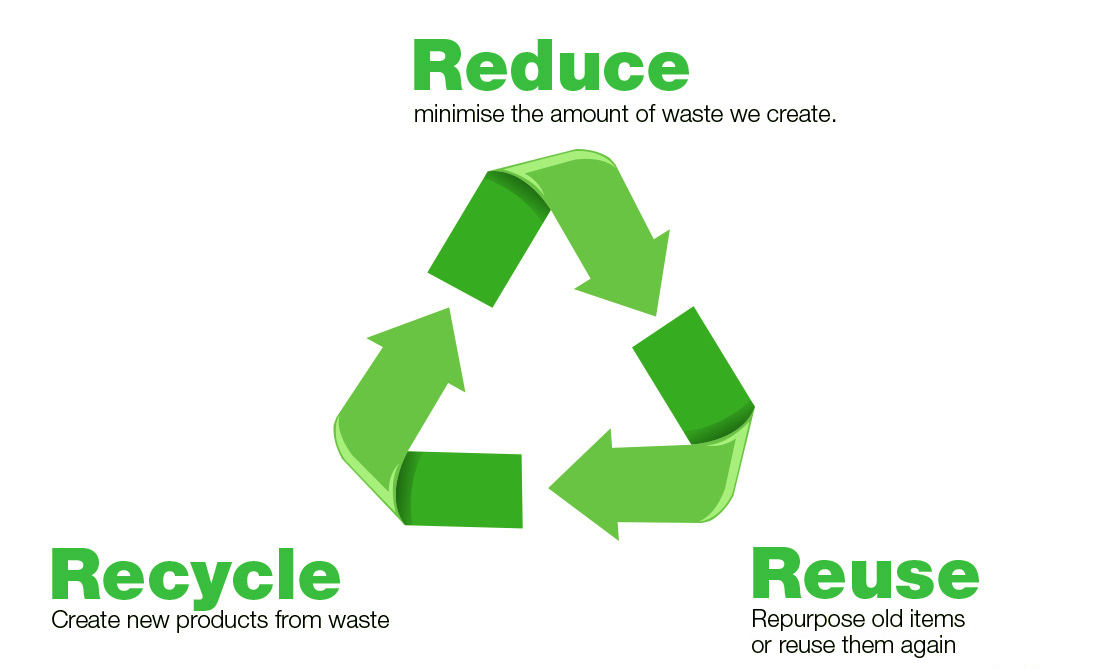
\includegraphics[width=0.7\linewidth]{3R-reduce-reuse-recycle.jpg}
        \caption[Prinzip: Reduce, Reuse, Recycle]{Prinzip: Reduce, Reuse, Recycle \footnotemark}
        
        \label{fig:3R}
    \end{figure} 

    \footnotetext{Quelle: \url{https://innovation-yachts.com/3r-reduce-reuse-recycle/}}

Nachhaltigkeit spielt eine zunehmend zentrale Rolle in der Produktentwicklung, insbesondere im Bereich Maschinenbau und Automation. In unserem Projekt im Modul Pren1 haben wir die Prinzipien der Nachhaltigkeit bewusst berücksichtigt, um einen positiven Beitrag zur Umwelt zu leisten und die Ressourcennutzung zu optimieren.

\subsection{Reduce – Ressourcen minimieren}

Ein Schwerpunkt unserer Arbeit lag darauf, den Materialverbrauch und den Energiebedarf zu reduzieren. Bereits in der Konzeptentwicklung wurden ressourceneffiziente Designs gesucht, welche mit möglichst wenig Komponenten zurechtkommen, um den Materialeinsatz so gering wie möglich zu halten. Dabei wurde ein grosses Augenmerk auf die Einsparung von Elektrokomponenten gelegt, so haben wir uns für ein Konzept entschieden, welches mit lediglich zwei Fahrantrieben und nur einem Antrieb für die gesamte Hindernisbewältigung auskommt. Durch ein rein mechanisches System können auch Sensoren eingespart werden, welche die einzelnen Schritte bei der Hindernisbewältigung auf Erfüllung überprüfen, bevor der nächste Schritt ausgelöst wird. Auch beim Prototyping wurde darauf geachtet, nur Teile herzustellen, welche wir effektiv für nötig hielten. 

\subsection{Reuse – Wiederverwendbarkeit fördern}

Ein weiteres Ziel war es, die Wiederverwendbarkeit der Komponenten zu erhöhen. Modulare Bauweisen und standardisierte Schnittstellen wurden implementiert, um eine einfache Demontage und Wiederverwendung einzelner Bauteile zu ermöglichen. Bevor Bauteile bestellt wurden, haben wir jeweils abgeklärt, ob diese von früheren Pren-Durchführungen geerbt werden können. Speziell bei Testaufbauten wurde darauf geachtet, wenn möglich, bereits vorhandene Teile zu verwenden, beispielsweise bei Fahrtests ein Chassis aus einem alten Stück Holz zu verwenden, anstelle eines Chassis zu drucken.

\subsection{Recycle – Wiederverwertung ermöglichen}

Bei der Materialauswahl haben wir auf recyclingfähige Materialien geachtet, um eine umweltgerechte Entsorgung sicherzustellen. Die Vermeidung von Verbundwerkstoffen und der Einsatz sortenreiner Materialien erleichtern die Rückgewinnung und Wiederverwertung am Ende der Produktlebensdauer. Gleichzeitig haben wir bei der Entwicklung darauf geachtet, möglichst wenig Produktionsabfälle zu generieren, und diese gezielt dem Recycling zuzuführen.

\subsection{Ergebnis Nachhaltigkeit}

Durch die Integration der Prinzipien \textbf{Reduce, Reuse, Recycle} \ref{fig:3R} ist es möglich, die Nachhaltigkeit eines Produktes zu verbessern. Die Umsetzung dieser Strategien hat nicht nur ökologische Vorteile, sondern trägt auch zur Kostenreduktion bei. Dieses Projekt zeigt, dass nachhaltige Entwicklung und technologische Innovation Hand in Hand gehen können und müssen, um langfristig einen Mehrwert zu schaffen.

Diese Reflexion verdeutlicht, dass Nachhaltigkeit nicht nur ein Ziel, sondern ein integraler Bestandteil des Entwicklungsprozesses ist, den wir auch in Pren2 konsequent weiterverfolgen wollen.


\end{document}